\documentclass[]{DINOReportMemo}
\usepackage{DINO_C-REx}
\usepackage{colortbl}


\newcommand{\ModuleName}{Image Generation} %edit this!
\newcommand{\subject}{Systems Engineering Report: Camera Model Time Integration Study} %edit this!
\newcommand{\status}{Initial Version}
\newcommand{\preparer}{Matt Muszynski} %edit this!
\newcommand{\summary}{Description, analysis, and recommendation for performing time integration of images taken during a spacecraft slew in such a way as to avoid non-physical artifacts in final simulated images.} %edit this
\usepackage{float}
\usepackage{rotating}
\usepackage{pdflscape}

\begin{document}

\makeCover


%
% enter the revision documentation here
% to add more lines, copy the table entry and the \hline, and paste after the current entry.
%
\pagestyle{empty}
{\renewcommand{\arraystretch}{2}
\noindent
\begin{longtable}{|p{0.5in}|p{4.5in}|p{1.14in}|}
\hline
{\bfseries Rev}: & {\bfseries Change Description} & {\bfseries By} \\
\hline
1.0 & Initial Release & Matt Muszynski \\ %edit this
\hline

\end{longtable}
}

\newpage
\setcounter{page}{1}
\pagestyle{fancy}

\tableofcontents
~\\ \hrule ~\\

\newpage
\section{Overview}\\\\
During a discussion between the DINO C-REx Systems Engineer and the Camera Team lead, a concern arose over the way the camera model should perform time integration. Currently, the camera model achieves time integration by summing a series of discrete scenes for each frame of an image. There is a concern that if spacecraft attitude rates are too high and the integration time step too low, the current method could introduce non-physical artifacts into simulated images. This document seeks to quantify the problem with a worse-case analysis and provides recommendations for mitigating the issue. 
\section{Method} \\
This document begins by a worst-case camera parameters including field of view, resolution, and attitude rate. It then attempts to quantify the maximum allowable time step that will result in objects travelling no more than 0.1 pixels between each scene. Cameras considered range as described in table \ref{min_max_params}.

\begin{table}
\centering
\caption{Minimum and Maximum Camera Parameters Studied}
\label{max_min_params}
\begin{tabular}{|l|l|l|}
\hline
Parameter     & Minimum & Maximum \\ \hline
Field of view & 2^\circ \times 2^\circ       & 10^\circ \times 10^\circ      \\ \hline
Resolution    & 512 \times 512     & 2048 \times 2048    \\ \hline
Slew Rate     & 0.05^\circ/sec     & 2^\circ/sec     \\ \hline
\end{tabular}
\label{min_max_params}
\end{table}
\section{Assumptions}
\begin{enumerate}
    \item The worst case (smallest) field of view modeled by DINO C-REx will be $2^\circ\times 2^\circ$.
    \item The worst cast (highest) resolution CCD modeled by DINO C-REx will be $2048\times2048$.
    \item The worst case (greatest) attitude rate while taking an image will be $2^\circ/sec$
    \item A point source that moves $<0.1$ pixels between time steps will not cause a non-physical artifact. (same assumption made in point spread model)
    \item Due to the constraints of the point spread model, all objects are modeled as either point sources or collections of point sources.
\end{enumerate}

\section{Calculation of Time Step}
The quantity we are most concerned with here is slew rate in terms of pixels/second. This is solved by finding the filed of view of an individual pixel dividing that by the number of degrees per pixel.
\begin{equation}
   {}^\circ/\text{pix} =  \frac{FOV (\text{in degrees})}{\text{pixel resolution}}
\end{equation}
\begin{equation}
   \text{slew rate in pixels} = \frac{\text{slew rate in degrees}}{{}^\circ/\text{pix}}
\end{equation}
Next, the number of pixels the camera slews through in a single time step $dt$ is given by:
\begin{equation}
    \frac{\text{pix}}{\text{s}}\cdot dt
\end{equation}
By setting the number of pixels the camera slews through in a times step to 0.1, we find an expression for the smallest acceptable time step for a given camera:
\begin{equation}
    dt = \frac{0.1}{\text{pix/s}} = \frac{0.1(\text{FOV in Degrees})}{(\text{resolution})(\text{slew rate in degrees per second})}
\end{equation}

\section{Time Step Plots}\\
Figures \ref{512} through \ref{2048} show plots of the number of pixels through which the camera slews and the maximum acceptable time step for a variety of camera resolutions, fields of view, and spacecraft slew rates. The results span from trivially workable to potentially problematic. The worst case scenario plotted (a $2^\circ$ FOV camera with $2048\times2048$ resolution, and a camera slew rate of $2^\circ/s$) would require a time step of just under 0.1ms.

\begin{figure*}[t!]
    \centering
    \begin{subfigure}
        \centering
        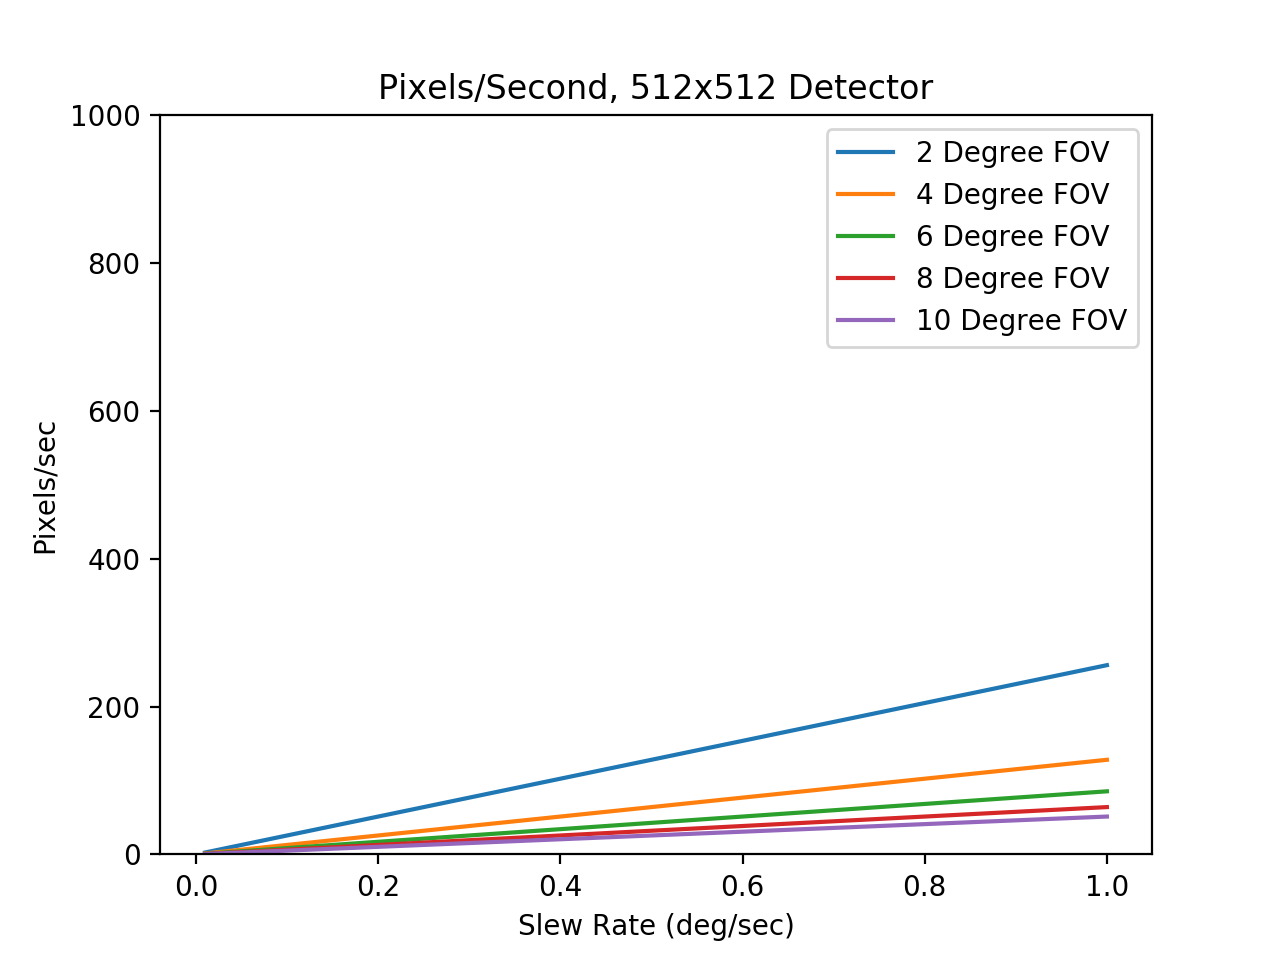
\includegraphics[height=2.1in]{512x512_pix_per_sec}
    \end{subfigure}%
    ~ 
    \begin{subfigure}
        \centering
        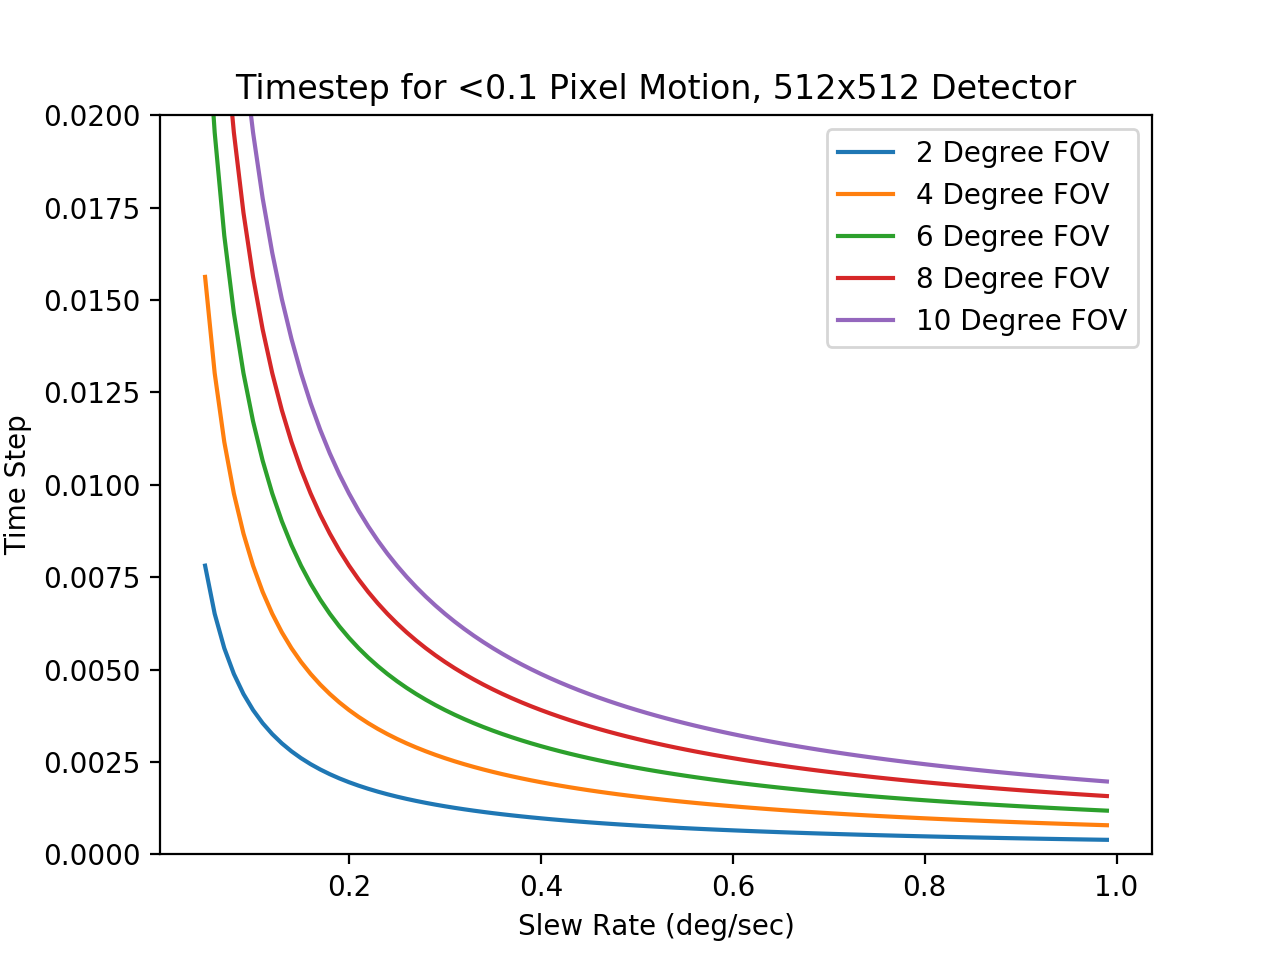
\includegraphics[height=2.1in]{512x512_min_dt}
    \end{subfigure}
    \caption{Best case plots show many solutions for $512\times512$ camera.}
    \label{512}
\end{figure*}


\begin{figure*}[t!]
    \centering
    \begin{subfigure}
        \centering
        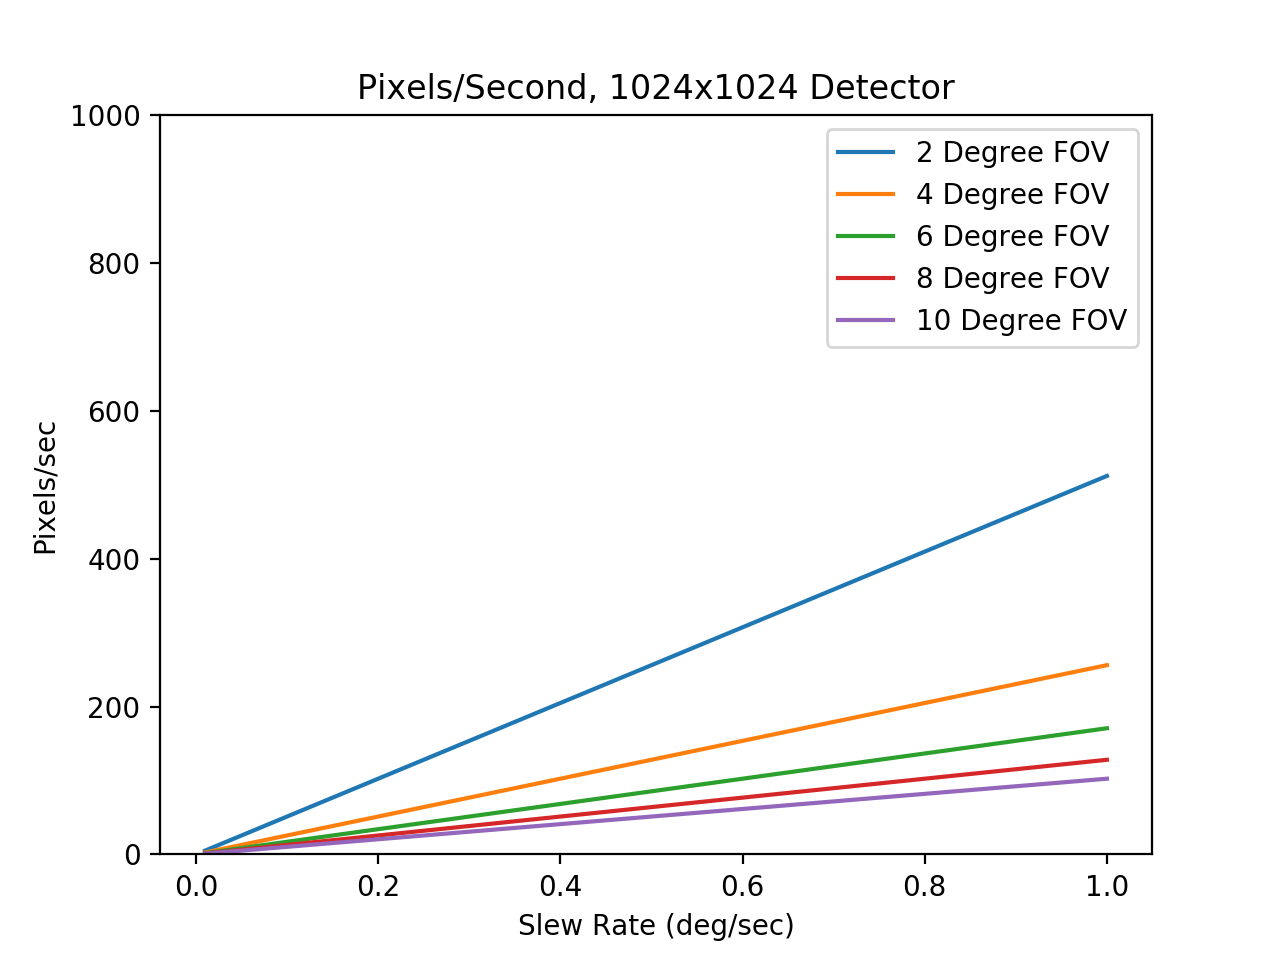
\includegraphics[height=2.1in]{1024x1024_pix_per_sec}
    \end{subfigure}%
    ~ 
    \begin{subfigure}
        \centering
        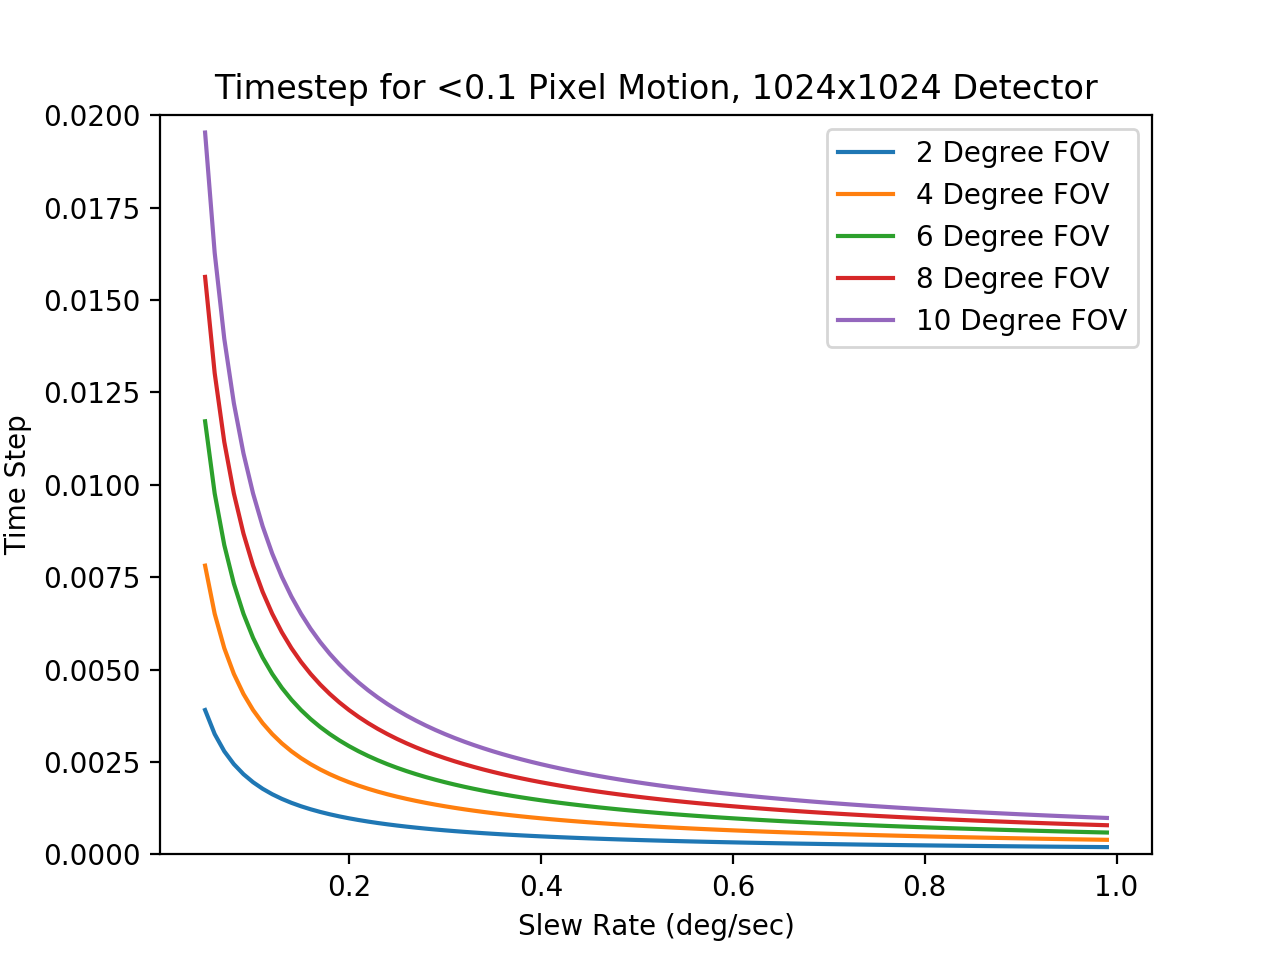
\includegraphics[height=2.1in]{1024x1024_min_dt}
    \end{subfigure}
    \caption{Same plots for worst case resolution of $2048\times2048$}
    \label{1024}
\end{figure*}


\begin{figure*}[t!]
    \centering
    \begin{subfigure}
        \centering
        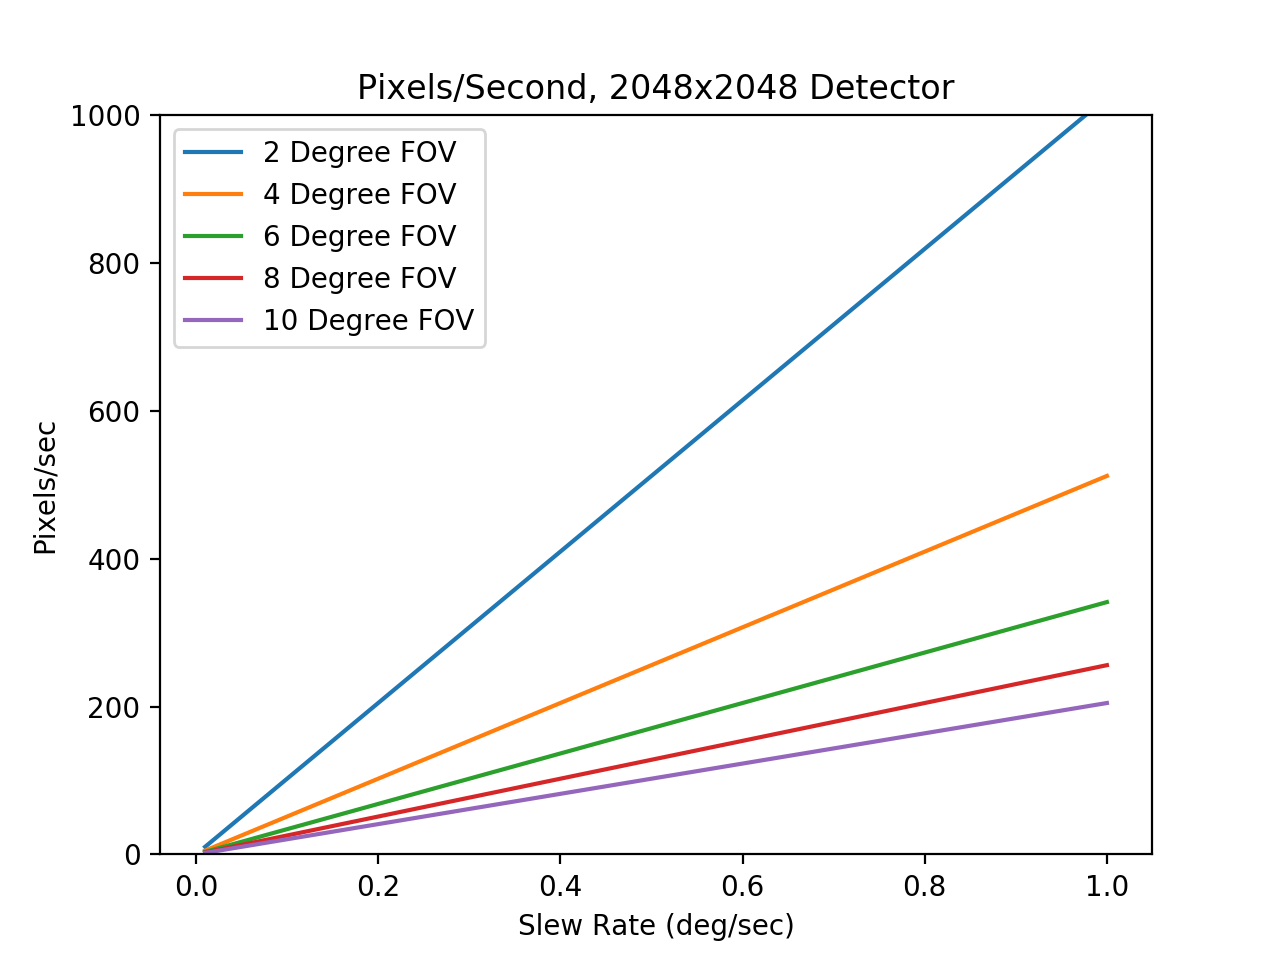
\includegraphics[height=2.1in]{2048x2048_pix_per_sec}
    \end{subfigure}%
    ~ 
    \begin{subfigure}
        \centering
        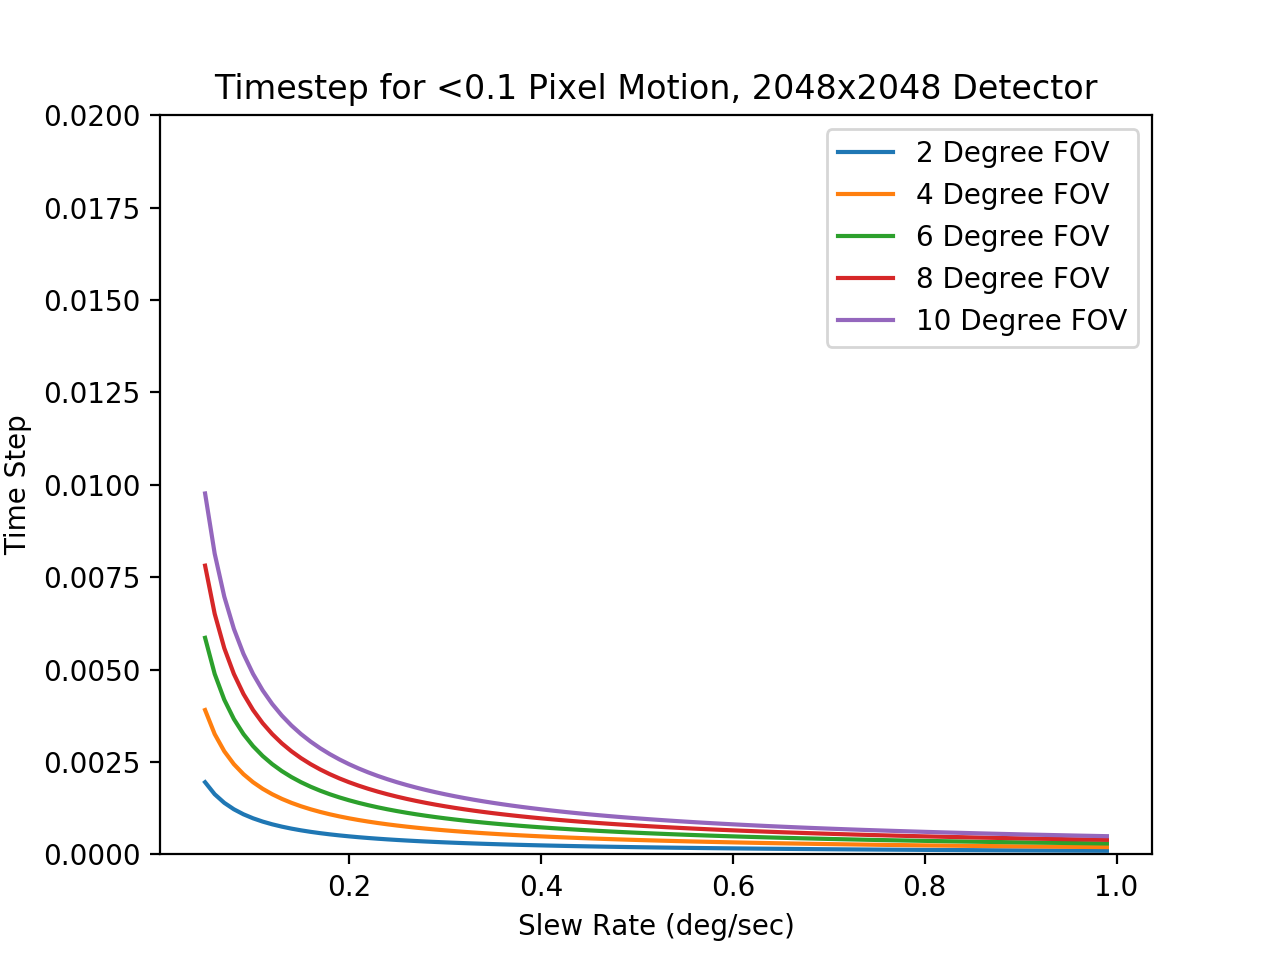
\includegraphics[height=2.1in]{2048x2048_min_dt}
    \end{subfigure}
    \caption{Even for the worst case resolution of $2048\times2048$, viable solutions exist for larger cameras and smaller slew rates.}
    \label{2048}
\end{figure*}

\section{Time Step Table}\\
Tables \ref{512_table} through \ref{2048_table} show the same data as figures \ref{512} through \ref{2048}. Although no minimum acceptable time step is yet defined, here we colorize any time steps below 1ms in red to illustrate a possible use case.

\begin{table}[]
\centering
\caption{Minimum acceptable integration times in seconds for $512\times512$ CCD (best case)}
\label{512_table}
\begin{tabular}{lc|c|c|c|c|c|c|c|c|}
\cline{3-10}
                                                          & \multicolumn{1}{c|}{} & \multicolumn{8}{c|}{Slew Rate (degrees per second)}                                                                                                                                                                                                    \\ \cline{3-10} 
                                                          &                       & 0.25     & 0.50                            & 0.75                            & 1.00                            & 1.25                            & 1.50                            & 1.75                            & 2.00                            \\ \hline
\multicolumn{1}{|l|}{}                                    & 2^\circ                     & 1.56e-03 & {\color[HTML]{FE0000} 7.81e-04} & {\color[HTML]{FE0000} 5.21e-04} & {\color[HTML]{FE0000} 3.91e-04} & {\color[HTML]{FE0000} 3.13e-04} & {\color[HTML]{FE0000} 2.60e-04} & {\color[HTML]{FE0000} 2.23e-04} & {\color[HTML]{FE0000} 1.95e-04} \\ \cline{2-10} 
\multicolumn{1}{|l|}{}                                    & 4^\circ                     & 3.13e-03 & 1.56e-03                        & 1.04e-03                        & {\color[HTML]{FE0000} 7.81e-04} & {\color[HTML]{FE0000} 6.25e-04} & {\color[HTML]{FE0000} 5.21e-04} & {\color[HTML]{FE0000} 4.46e-04} & {\color[HTML]{FE0000} 3.91e-04} \\ \cline{2-10} 
\multicolumn{1}{|l|}{}                                    & 6^\circ                     & 4.69e-03 & 2.34e-03                        & 1.56e-03                        & 1.17e-03                        & {\color[HTML]{FE0000} 9.37e-04} & {\color[HTML]{FE0000} 7.81e-04} & {\color[HTML]{FE0000} 6.70e-04} & {\color[HTML]{FE0000} 5.86e-04} \\ \cline{2-10} 
\multicolumn{1}{|l|}{}                                    & 8^\circ                     & 6.25e-03 & 3.13e-03                        & 2.08e-03                        & 1.56e-03                        & 1.25e-03                        & 1.04e-03                        & {\color[HTML]{FE0000} 8.93e-04} & {\color[HTML]{FE0000} 7.81e-04} \\ \cline{2-10} 
\multicolumn{1}{|l|}{{\rotatebox[origin=c]{90}{Resolution}}} & 10^\circ                    & 7.81e-03 & 3.91e-03                        & 2.60e-03                        & 1.95e-03                        & 1.56e-03                        & 1.30e-03                        & 1.12e-03                        & {\color[HTML]{FE0000} 9.77e-04} \\ \hline
\end{tabular}
\end{table}

\begin{table}[]
\centering
\caption{Minimum acceptable integration times in seconds for $1024\times1024$ CCD (intermediate case)}
\label{1024_table}
\begin{tabular}{ll|l|l|l|l|l|l|l|l|}
\cline{3-10}
                                                          &    & \multicolumn{8}{c|}{Slew Rate (degrees per second)}                                                                                                                                                                                                                           \\ \cline{3-10} 
                                                          &    & 0.25                            & 0.50                            & 0.75                            & 1.00                            & 1.25                            & 1.50                            & 1.75                            & 2.00                            \\ \hline
\multicolumn{1}{|l|}{}                                    & 2^\circ  & {\color[HTML]{FE0000} 7.81e-04} & {\color[HTML]{FE0000} 3.91e-04} & {\color[HTML]{FE0000} 2.60e-04} & {\color[HTML]{FE0000} 1.95e-04} & {\color[HTML]{FE0000} 1.56e-04} & {\color[HTML]{FE0000} 1.30e-04} & {\color[HTML]{FE0000} 1.12e-04} & {\color[HTML]{FE0000} 9.77e-05} \\ \cline{2-10} 
\multicolumn{1}{|l|}{}                                    & 4^\circ  & 1.56e-03                        & {\color[HTML]{FE0000} 7.81e-04} & {\color[HTML]{FE0000} 5.21e-04} & {\color[HTML]{FE0000} 3.91e-04} & {\color[HTML]{FE0000} 3.13e-04} & {\color[HTML]{FE0000} 2.60e-04} & {\color[HTML]{FE0000} 2.23e-04} & {\color[HTML]{FE0000} 1.95e-04} \\ \cline{2-10} 
\multicolumn{1}{|l|}{}                                    & 6^\circ  & 2.34e-03                        & 1.17e-03                        & {\color[HTML]{FE0000} 7.81e-04} & {\color[HTML]{FE0000} 5.86e-04} & {\color[HTML]{FE0000} 4.69e-04} & {\color[HTML]{FE0000} 3.91e-04} & {\color[HTML]{FE0000} 3.35e-04} & {\color[HTML]{FE0000} 2.93e-04} \\ \cline{2-10} 
\multicolumn{1}{|l|}{}                                    & 8^\circ  & 3.13e-03                        & 1.56e-03                        & 1.04e-03                        & {\color[HTML]{FE0000} 7.81e-04} & {\color[HTML]{FE0000} 6.25e-04} & {\color[HTML]{FE0000} 5.21e-04} & {\color[HTML]{FE0000} 4.46e-04} & {\color[HTML]{FE0000} 3.91e-04} \\ \cline{2-10} 
\multicolumn{1}{|l|}{{\rotatebox[origin=c]{90}{Resolution}}} & 10^\circ & 3.91e-03                        & 1.95e-03                        & 1.30e-03                        & {\color[HTML]{FE0000} 9.77e-04} & {\color[HTML]{FE0000} 7.81e-04} & {\color[HTML]{FE0000} 6.51e-04} & {\color[HTML]{FE0000} 5.58e-04} & {\color[HTML]{FE0000} 4.88e-04} \\ \hline
\end{tabular}
\end{table}

\begin{table}[]
\centering
\caption{Minimum acceptable integration times in seconds for $2048\times2048$ CCD (worst case)}
\label{2048_table}
\begin{tabular}{ll|l|l|l|l|l|l|l|l|}
\cline{3-10}
                                                          &    & \multicolumn{8}{c|}{Slew Rate (degrees per second)}                                                                                                                                                                                                                           \\ \cline{3-10} 
                                                          &    & 0.25                            & 0.50                            & 0.75                            & 1.00                            & 1.25                            & 1.50                            & 1.75                            & 2.00                            \\ \hline
\multicolumn{1}{|l|}{}                                    & 2^\circ  & {\color[HTML]{FE0000} 3.91e-04} & {\color[HTML]{FE0000} 1.95e-04} & {\color[HTML]{FE0000} 1.30e-04} & {\color[HTML]{FE0000} 9.77e-05} & {\color[HTML]{FE0000} 7.81e-05} & {\color[HTML]{FE0000} 6.51e-05} & {\color[HTML]{FE0000} 5.58e-05} & {\color[HTML]{FE0000} 4.88e-05} \\ \cline{2-10} 
\multicolumn{1}{|l|}{}                                    & 4^\circ  & {\color[HTML]{FE0000} 7.81e-04} & {\color[HTML]{FE0000} 3.91e-04} & {\color[HTML]{FE0000} 2.60e-04} & {\color[HTML]{FE0000} 1.95e-04} & {\color[HTML]{FE0000} 1.56e-04} & {\color[HTML]{FE0000} 1.30e-04} & {\color[HTML]{FE0000} 1.12e-04} & {\color[HTML]{FE0000} 9.77e-05} \\ \cline{2-10} 
\multicolumn{1}{|l|}{}                                    & 6^\circ  & 1.17e-03                        & {\color[HTML]{FE0000} 5.86e-04} & {\color[HTML]{FE0000} 3.91e-04} & {\color[HTML]{FE0000} 2.93e-04} & {\color[HTML]{FE0000} 2.34e-04} & {\color[HTML]{FE0000} 1.95e-04} & {\color[HTML]{FE0000} 1.67e-04} & {\color[HTML]{FE0000} 1.46e-04} \\ \cline{2-10} 
\multicolumn{1}{|l|}{}                                    & 8^\circ  & 1.56e-03                        & {\color[HTML]{FE0000} 7.81e-04} & {\color[HTML]{FE0000} 5.21e-04} & {\color[HTML]{FE0000} 3.91e-04} & {\color[HTML]{FE0000} 3.13e-04} & {\color[HTML]{FE0000} 2.60e-04} & {\color[HTML]{FE0000} 2.23e-04} & {\color[HTML]{FE0000} 1.95e-04} \\ \cline{2-10} 
\multicolumn{1}{|l|}{{\rotatebox[origin=c]{90}{Resolution}}} & 10^\circ & 1.95e-03                        & {\color[HTML]{FE0000} 9.77e-04} & {\color[HTML]{FE0000} 6.51e-04} & {\color[HTML]{FE0000} 4.88e-04} & {\color[HTML]{FE0000} 3.91e-04} & {\color[HTML]{FE0000} 3.26e-04} & {\color[HTML]{FE0000} 2.79e-04} & {\color[HTML]{FE0000} 2.44e-04} \\ \hline
\end{tabular}
\end{table}
\pagebreak
\section{Recommendations}  \\
The acceptability of the findings presented in this SER will depend on buy in from multiple parties, most importantly the DINO C-REx Systems Engineer and Basilisk specialist Andrew Harris. Specific recommendations are made below.
    \subsection{Define A Minimum Acceptable Time Step} \\Due to processing constraints, there should be some absolute minimum acceptable time step that may be a function of the total number of discrete scenes that must be computed per integrated image. This will depend highly on the time it takes to process each scene.
    \subsection{Define A Maximum Acceptable Slew Rate During an Image} \\
    Defining the maximum acceptable slew rate will also inform this study profoundly. If the maximum slew rate during an image is small enough, any camera configuration will likely lead to an acceptable integration time step. However, it is important to note here that this maximum rate must by driven by simulation parameters and not by a need to make the camera model work. If the maximum desired slew rate drives unacceptable camera outcomes, the team must work to find a different way to solve the problem.
    \subsection{Define Maximum Resolution and Minimum Field of View}\\
    Because the worst performing camera configurations are those with large resolutions and small fields of view, the Camera team should work with the customer to develop a maximum resolution and a minimum field of view that is acceptable for the project. This should be informed by available cubesat hardware.
    \subsection{Optimize Camera Code}\\
    If discussions with the Systems Engineer prove that desired camera/slew rate configurations conflict with the minimum acceptable time step, further efforts could be made to optimize the camera code. For example, computing stars in the camera FOV is currently done at every time step. The system could reduce the number of stars it must handle at each step by defining a nominal attitude for the image and creating a temporary star catalog once per image that would include all stars in the FOV of the camera at its nominal attitude plus some buffer to acount for stars that come into view as the camera slews across the sky.
    \subsection{Optimize Image Generation} \\
    Another optimization tactic that could be used would be to make the entire image only \textit{after} the attitude simulation has finished. A process will tell the camera when it should be taking an image. The most efficient way to handle smearing could be to simply track the pattern the camera boresight traces in the sky. Then, only when the camera is told that it should stop taking the image, it uses the pattern traced by the boresight to "stamp" on each star/facet similar to the way the system currently handles PSF. The same time step concerns described above still apply, but this would likely drastically improve processing speed.
    \subsection{Rework Camera Code to Leverage Basilisk Integration Methods}\\
    This recommendation has the lowest desirability of all presented in the SER, but it is included because it may be necessary. If no acceptable minimum/maximum parameters can be agree upon, the camera code may need to be reworked to be integrated with the Basilisk integration engine. This will likely require significant rework and although it remains an option, all efforts should be made to solve the problem through other means.

\end{document}
